\documentclass[10pt, a4paper]{beamer}

\usetheme{Berkeley}
\usecolortheme{sidebartab}
\usepackage{parskip}
\usepackage{graphicx}

\setlength{\parindent}{15pt}

\begin{document}
	\setbeamertemplate{sidebar left}{}
	\title{Progress Presentation-I}
	\subtitle{e-Yantra Summer Intership-2016 \\ Distributed Robotics - Multi Swarm Robots}
	\author{Chinmay C\\R Hariharan\\
	\textbf{Mentors}:\\ Ms. Rutuja and Ms. Deepa}
	\institute{IIT Bombay}
	\date{\today}
	%\addtobeamertemplate{sidebar left}{}{\includegraphics[scale = 0.3]{logowithtext.png}}
	\frame{\titlepage}

\setbeamertemplate{sidebar left}[sidebar theme]
\section{Overview of Project}
\begin{frame}{Overview of Project}
	\begin{itemize}
		\setlength\itemsep{0em}
		\item \textbf{Project Name}
			\begin{itemize} 
				\setlength\itemsep{-1em}
				\item Distributed Robotics - Multi Swarm Robots
			\end{itemize}
		\item \textbf{Objective} 
			\begin{itemize}
				\setlength\itemsep{-0.7em}
				\item \textbf{Bulid minibots} which have capabilities to sense its surrounding and communicate with its neighbouring robots
				\item \textbf{Shape formation} using the minibots
			\end{itemize}
		\item \textbf{Deliverables}
			\begin{itemize}
				\setlength\itemsep{-0.7em}
				\item \textbf{Five Minibots} that can portray swarm behaviours 
				\item Implement/Develop an \textbf{algorithm} to form shapes using the robots
			\end{itemize}
	\end{itemize}
\end{frame}

\section{Overview of Task}
\begin{frame}{Overview of Task}
	\begin{center}
		\begin{tabular}{|p{8cm}|p{1cm}|} 
			\hline
			\textbf{TASK} & \textbf{DAYS} \\ 
			\hline
			Study the concepts of swarm robotics and get familiar with different robots available & 3 \\ 
			\hline
			Make the Minibots: & \\ 
			\hline
			Study the kinematics of differential drive configuration & 3 \\ 
			\hline
			Select appropriate sensors to be added: & 3 \\ 
			\hline
			Design the pcbs & 3 \\ 
			\hline
			Assemble all the components & 4 \\ 
			\hline
			Test the robots & 3 \\ 
			\hline
			Solve rendezvous problem using homogenous controller gain & 2 \\ 
			\hline
			Solve rendezvous problem using heterogenous controller gain & 2 \\ 
			\hline
			Shape formation & 4 \\ 
			\hline
			Documentation & 5 \\ 
			\hline		
		\end{tabular}
	\end{center}
\end{frame}

\section{Task Accomplised}
\begin{frame}{Task Accomplised}
	\begin{itemize}
		\setlength\itemsep{-0.5em}
		\item Understanding the fundamentals of swarm robotics
		\item Learning motion kinematics and inverse kinematics for mapping distance and angle to the position
		\item Designing PCB:
		\begin{itemize}
			\setlength\itemsep{-1em}
			\item Components and shape (8cm dia) finalization
			\item Understanding eagle software
			\item Designing schematics
			\item Placing parts in PCB layout
			\item Routing the PCB, generating Bill of materials and gerber files
			\item Finalizing PCB design
		\end{itemize}
		\item Solved rendezvous problem using Firebird V robots
		\item Developed an algorithm for line formation by swarm robots
	\end{itemize}
\end{frame}

\section{Basic Design of Minibot}
\begin{frame}{Basic Desgin of Minibot}
	\begin{figure}
		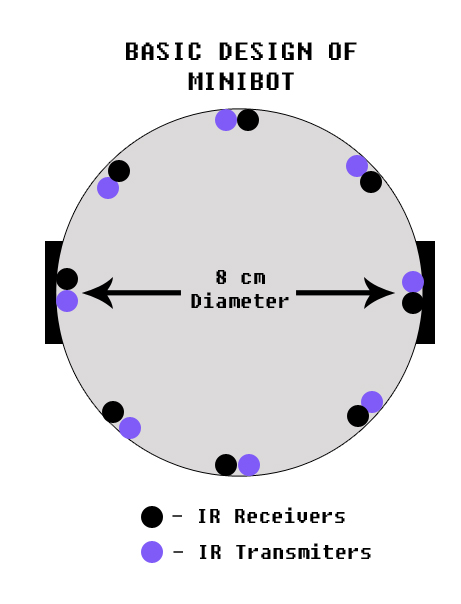
\includegraphics[width=160px]{basic_design.jpg}
		\label{fig:Design}
	\end{figure}
\end{frame}

\section{PCB Design and Schematics}
\begin{frame}{PCB Design and Schematic}
\begin{figure}
	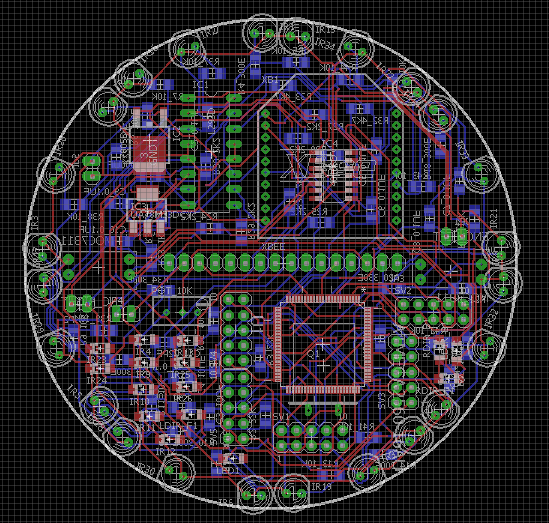
\includegraphics[width=220px]{PCB_design_layout.png}
	\label{fig:PCB Design}
\end{figure}
\end{frame}


\section{Challenges Faced}
\begin{frame}{Challenges Faced}
	\begin{itemize}
		\item Miniaturizing the design of minirobot
		\item Designing of PCB with the constraints in size
		\item Routing double layered PCB
		\item Mapping IR reading to actual distances
		\item Designing line formation algorithm with respect to relative positions of robots
	\end{itemize}
\end{frame}

\section{Future Plans}
\begin{frame}{Future Plans}
	\begin{itemize}
		\item Desinging and building chassis for the minibots
		\item Printing of PCB and soldering parts
		\item Reading on already existing shape forming algorithms in swarm robots
		\item Developing an algorithm for forming regular shapes
		\item Further implementing the same for alphabets
	\end{itemize}
\end{frame}


\section{Thank You}
\begin{frame}{Thank You}
	\begin{tabular}{p{3cm} c c}
	 	& THANK YOU !!! &
	\end{tabular}
\end{frame}
\end{document}
